\documentclass
[
%draft,						% don't render pictures, for speed
a4paper,                      % Format A4
twoside,					  % double sided, alternative: oneside
11pt,                         % font size
abstract,		      % include if you want to use the abstract environment (if there is an abstract)
%fleqn,                        % equations are aligned on the left side, comment if you want centered equations
%BCOR=5mm,                     % indention on left side because of the binding
%cleardoubleplain              % page numbers are printed on empty pages, comment if this is not desired
]
{scrartcl} % KOMA script package for scientific articles
%-----------------------------------------------------------------------------------
% Packages (do not touch if you don't know what you are doing)
%-----------------------------------------------------------------------------------
% symbols and orthography
\usepackage{blindtext}			% enables you to create blindtext (lorem ipsum ...)
\usepackage[utf8]{inputenc} % symbol set 
\usepackage[english]{babel}   	% englisch orthography
%\usepackage[french]{babel}	   % french					
%\usepackage[ngerman]{babel}   % german
\usepackage[T1]{fontenc}      % enables "Umlaute" (not really needed for English)
\usepackage[scaled=.90]{helvet}
\usepackage{datetime}
%----------------------
% graphics
\usepackage{graphicx}         	% package to include graphics (pdf, png, jpg)
\usepackage{subfig}			% package for subfigures
\usepackage{float}            		% Option [H] for fixing floats where you want them to be (not recommended unless you really need it)
\usepackage[section]{placeins} 		% keep floats within floatBarrier
%------------------------------
% math packages
%\usepackage[cmex10]{amsmath}  
\usepackage{amsmath} 
\usepackage{amstext}          % for Klartext via \text{} in Formeln
\usepackage{amsfonts}         % for komplexere Formeln (Mengensymbole ...)
\usepackage{amssymb}          % for komplexere Formeln (Mengensymbole ...)
\usepackage{bm}               % bold math use \bm{}
\usepackage{gensymb}

%--------------------------------
% other packages
\usepackage{enumerate}        	% better listings
\usepackage{listings}		  	% include source code
\usepackage{booktabs}         	% nicer tables (see manual for usage)
\usepackage{colortbl,color,xcolor}
\usepackage{textcomp}        	% for \textdegree , \textcelsius
%\usepackage{algorithm}        % for including algorithms
%\usepackage{algorithmic}      % same as above, but other package (check the manual for usage) 
%\usepackage{theorem}          % for theorems
%\usepackage{todonotes}
\usepackage{pdfpages}         % include whole pages from pdf files
\usepackage{parskip}          % insert an empty line between paragraphs instead of an indented beginning
\usepackage[right]{eurosym}   % Euro symbol
\usepackage[hyphens]{url}     %enables line breaks for URLs \url{http://www}
% set border size of page (comment if you want Latex to do this)
\usepackage[inner=5cm,%
								outer=2cm,%
								top=2.7cm,%
								bottom=3.2cm]{geometry}
\usepackage{setspace}		  % for a different line spacing
%-----------------------------------------------------------------------------------
% other stuff (do not touch, it is good that way !)
%-----------------------------------------------------------------------------------
\sloppy                   % avoids lines that are too long on the right side
% avoid "orphans"
\clubpenalty = 10000
% avoid "widows"
\widowpenalty = 10000
% this makes the table of content etc. look better
\renewcommand{\dotfill}{\leaders\hbox to 5pt{\hss.\hss}\hfill}

% avoid indentation of line after a paragraph
\setlength{\parindent}{0pt}

% label equations with (section-number.equation.number)
\numberwithin{equation}{section}

\renewcommand{\textfraction}{0.05}
\renewcommand{\topfraction}{0.8}
\renewcommand{\bottomfraction}{0.8}
\renewcommand{\floatpagefraction}{0.75}
%-----------------------------------------------------------------------------------
%-----------------------------------------------------------------------------------

% Header and footer settings
% 
\usepackage[headsepline, footsepline]{scrlayer-scrpage} % see manual for usage
\automark[section]{section}
\ofoot{\pagemark} % ofoo
%\ifoot{SOMETHING} % ofoo
%\cfoot[]{\pagemark}
%\ihead{}
%\ohead{}
%\ohead{\headmark}
% \setheadsepline{0.5pt}
% \setfootsepline{0.5pt}

%%%%%%%%%%%%%%%%%%%%%%%%%%%%%%%%%%%%%%%%%%%%%%%%%%%%%%%%%%%%%%%%%%%%%%%%%%%%%%%
%%%%%%%%%%%%%%%%%%%%%%%%%%%%%%%%%%%%%%%%%%%%%%%%%%%%%%%%%%%%%%%%%%%%%%%%%%%%%%
%
% References with BibTeX
%
\usepackage{natbib}
%\bibliographystyle{plain}
\bibliographystyle{apalike}
%\bibliographystyle{elsart-harv}
\setlength{\bibsep}{3mm}                  % spacing of the entries in the references
%
% look at the chapterbib package if you want to use a separate bibliography for each chapter
%
%%%%%%%%%%%%%%%%%%%%%%%%%%%%%%%%%%%%%%%%%%%%%%%%%%%%%%%%%%%%%%%%%%%%%%%%%%%%%%
%%%%%%%%%%%%%%%%%%%%%%%%%%%%%%%%%%%%%%%%%%%%%%%%%%%%%%%%%%%%%%%%%%%%%%%%%%%%%%
%
% some other stuff...
%
\setlength{\unitlength}{1cm}
\setlength{\oddsidemargin}{0.3cm}
\setlength{\evensidemargin}{0.3cm}
\setlength{\textwidth}{15.5cm}
\setlength{\topmargin}{0cm}
\setlength{\textheight}{22cm}
\columnsep 0.5cm
%%%%%%%%%%%%%%%%%%%%%%%%%%%%%%%%%%%%%%%%%%%%%%%%

% just compile particular parts
%
%\includeonly{./SUMMARY/summary} % put in here the path of the file you want to include only
%\includeonly{thesis_Ic1_intro}
%%%%%%%%%%%%%%%%%%%%%%%%%%%%%%%%%%%%%%%%%%%%%%%%%%%%%%%%%%%%%%%%%%%%%%%%%%%%%%

% define own commands
\newcommand{\brac}[1]{\left(#1\right)}
\newcommand{\todo}[1]{\textbf{\textsc{\textcolor{red}{(TODO: #1)}}}}
\newcommand{\pcode}[1]{\textcolor{blue}{#1}}
\newcommand{\scode}[1]{\textcolor{olivegreen}{#1}}
\newdateformat{monthyeardate}{\monthname[\THEMONTH] \THEYEAR}

%-----------------------------------------------------------------------------------
% STASRT OF THE ACTUAL DOCUMENT
%-----------------------------------------------------------------------------------
\begin{document}

\pagestyle{empty}

% Title page
\newgeometry{inner=3cm,outer=2cm,top=1.8cm,bottom=2.2cm}
\input{I3ELVIS_title}
\clearpage
\restoregeometry

\setcounter{page}{1}

\tableofcontents 

%\listoffigures
%\addcontentsline{toc}{chapter}{List of figures}
%\clearpage

%\listoftables
%\addcontentsline{toc}{chapter}{List of tables}
%\cleardoublepage

%\listofalgorithms
%\addcontentsline{toc}{chapter}{List of algorithms}




%
\onehalfspacing				% 1.5 line spacing
%\singlespacing				% single line spacing

\pagestyle{scrheadings}		% pagenumbering using the scrpage2 settings


%------------------------------------------------------------
% The following structure is not mandatory!!!!
%------------------------------------------------------------

% Abstract: if you want to put this in, you have to activate the abstract option at the top (documentclass options)

%\input{thesis_abstract_I}


% Introduction
%---------------------
% you can either write directly in here or use separate files that are then included using \include or \input (see manual for the difference between both)


%------------------------
% the physics/rheology of I3ELVIS
% Part II - chapter 2: Methods

\section{Physics}

\subsection{Basic physical principals}

\subsubsection{The continuity equation}

% continuity equ.
The continuity equation describes the conservation of mass, while it is displaced in a continuous medium. In its Lagrangian form it reads the following,

\begin{equation}\label{eqs:cont_general}
\dfrac{D \rho}{D t} + \rho \nabla\cdot\vec{v} = 0,
\end{equation}

where $\rho$ denotes material density, $\vec{v}$ denotes displacement velocity and $\dfrac{D}{D t}$ denotes the Lagrangian time derivative.

For many geological media like the crust or the mantle, where temperature and pressure are not too large and no phase changes occur, which would lead to larger volume changes, one can assume the following \textit{incompressibility condition},

\begin{equation}\label{eqs:imcompress}
\dfrac{D \rho}{D t} = \dfrac{\partial \rho}{\partial t} +\vec{v} \nabla\rho = 0,
\end{equation}

which means that the density of material points does not change in time.

This leads us to the following \textit{incompressible continuity equation}, which is the same in its Eulerian and Lagrangian form,

\begin{equation}
\nabla\cdot\vec{v}=0,
\end{equation}

The \textit{incompressible continuity equation} very widely used in numerical geodynamic modelling, although it is often a rather strong simplification.

\subsubsection{The Navier-Stokes Euqation}

The Navier-Stokes equation of motion in its full form reads the following,

\begin{equation}\label{eqs:NS}
\dfrac{\partial \sigma'_{ij}}{\partial x_j} - \dfrac{\partial P}{\partial x_i} + \rho g_i = \rho \dfrac{D v_i}{D t},
\end{equation}

where $\sigma_{ij}$ is the strain-rate and $\vec{g} = \left(g_x,g_y,g_z\right)$ is the gravity vector.

In highly viscous flows the right-hand side of \eqref{eqs:NS}, the inertial forces $\rho \dfrac{D v_i}{D t}$, is much smaller compared to the gravitational force and therefore, be neglected. This leads to the \textit{Stokes equation for creeping flow},

\begin{equation}\label{eqs:Stokes}
\dfrac{\partial \sigma'_{ij}}{\partial x_j} - \dfrac{\partial P}{\partial x_i} + \rho g_i = 0.
\end{equation}

Under Boussinesq approximation the density is assumed to be constant, except in the buoyancy force term, where temperature and volatile content play an important role \citep{Gerya2003}. Taking into account the Boussinesq approximation, density $\rho(T, P, c)$ in the buoyancy term $\rho g_i$ may vary locally as a function of temperature $T$, pressure $P$ and composition $c$,

\begin{equation}\label{eqs:Boussinesq}
\dfrac{\partial \sigma'_{ij}}{\partial x_j} - \dfrac{\partial P}{\partial x_i} = - \rho(T, P, c) g_i.
\end{equation}

\subsubsection{Heat conservation equation}

The heat conservation equation, also called temperature equation, describes the heat balance in a convective medium, taking into account changes due to internal heat generation, advection and conduction. The Lagrangian heat conservation equation reads as follows,

\begin{equation}
\rho C_p \left(\dfrac{D T}{D t}\right) = - \nabla \cdot \vec{q} + H_r + H_a + H_s + H_L,
\end{equation}

with $\vec{q} = -k(T, p, c) \nabla T$, where thermal conductivity $k(T, P, c)$ depends on temperature, pressure and rock composition $c$. $H_r, H_a, H_s, H_L$ denote radioactive, adiabatic, shear and latent heating.

Adiabatic and shear heating have shown to be important in many tectonic situations, which is why they are not taken as constant.

\begin{subequations}\label{eqs:extendedBoussinesq}
\begin{equation}
H_r = const.
\end{equation}
\begin{equation}
H_a = T \alpha \vec{v} \nabla P
\end{equation}
\begin{equation}
H_s = \sigma'_{ij} \left(\dot{\epsilon}'_{ij} - \dot{\epsilon}_{ij(elastic)} \right)
\end{equation}
\begin{equation}
H_L = const.
\end{equation}
\end{subequations}

The resulting set of the above equations, together with equations \eqref{eqs:Boussinesq} and \eqref{eqs:extendedBoussinesq}, is called the extended Boussinesq approximations.

\subsubsection{Rheology}

\paragraph{Equation of State}
% see code: mark3mg.c <dencalc()> l.945
\begin{equation}\label{eqs:EOS}
\rho = \rho_r  \left[ 1 + \beta \left( P - P_r \right) \right] \times \left[ 1 - \alpha \left( T - T_r \right) \right]
\end{equation}
where $\rho_r$ is the reference density given separately for each rock type, $P_r=1.0\,bar$ is the reference pressure, $T_r=298.15\,K$ is the reference temperature, $\alpha$ is the thermal expansion and $\beta$ is the compressibility.

\paragraph{Viscosity}
% see mark3mg.c <viscalc()>
\paragraph{Plastic yield strength}
\begin{equation}\label{eqs:mohr_coulomb}
\sigma_{yield} = C + sin(\phi_{dry})(1-\lambda) P
\end{equation}
where $\sigma_{yield}$ denotes the shear stress limit after which plastic yielding occurs, $C$ is the cohesion, $\phi_{dry}$ is the effective internal friction angle in dry rock, $\lambda=1-\dfrac{P_{fluid}}{P_{solid}}$ is the pore fluid pressure factor and $P=P_{solid}$ is the mean stress of the solid.

\paragraph{Peirl's creep (Katayamo \& Karato, 2008)}
\begin{equation}\label{eqs:peirls_strain_rate}
\dot{\epsilon}_{II} = A_{Peirl} \sigma_{II}^2 exp \left\lbrace -\dfrac{E_a + P V_a}{R T}  \left[ 1- \left( \dfrac{\sigma_{II}}{\sigma_{Peirl}} \right) ^k \right] ^q \right\rbrace
\end{equation}

For I3ELVIS, elasticity has not yet been implemented, thus the implemented rheology in three dimensions is visco-plastic (time of writing: December 14, 2020).
For I2ELVIS, a visco-elasto-plastic rheology is employed, with the deviatoric strain-rate $\dot{\epsilon}'_{ij}$ being composed of the following components,

\begin{equation}
\dot{\epsilon}'_{ij} = \dot{\epsilon}'_{ij(viscous)} + \dot{\epsilon}'_{ij(elastic)} + \dot{\epsilon}'_{ij(plastic},
\end{equation}

where

\begin{subequations}
\begin{equation}
\dot{\epsilon}'_{ij(viscous)} = \dfrac{1}{2 \eta} \sigma'_{ij},
\end{equation}
\begin{equation}
\dot{\epsilon}'_{ij(elastic)} = \dfrac{1}{2 \mu} \dfrac{D \sigma'_{ij}}{D t},
\end{equation}
\begin{equation}
\dot{\epsilon}'_{ij(plastic)} = \chi \dfrac{\partial G}{\partial \sigma'_{ij}} = \chi \dfrac{\sigma'_{ij}}{2 \sigma_{II}} \quad \text{for}\, G = \sigma_{II} = \sigma_{yield}.
\end{equation}
\end{subequations}

where $\eta$ denotes viscosity, $\sigma'_{ij}$ denotes the deviatoric stress tensor, $\mu$ denotes the shear modulus, $G$ is the plastic potential, $\sigma_{yield}$ is yield strength, $\sigma_{II}=\sqrt{\frac{1}{2}\sigma_{ij}^{'2}}$ is second deviatoric stress invariant and $\chi$ is plastic potential.
% stress and strain
Generally the strain tensor $\epsilon_{ij}$ can be defined as a function of displacement $\vec{u} = (u_x, u_y, u_z)$,

\begin{equation}\label{strain}
\epsilon_{ij} = \dfrac{1}{2} \left(\dfrac{\partial u_i}{\partial x_j} + \dfrac{\partial u_j}{x_i}\right).
\end{equation}
and the second strain rate invariant is given by $\dot{\epsilon}_{II} = \sqrt{\frac{1}{2}\dot{\epsilon}_{ij}^{'2}}$

The viscosity $\eta$ is defined as follows,

\begin{equation}
\eta = \left(\dfrac{2}{\sigma_{II}}\right)^{\left(n-1\right)}\dfrac{F^n}{A_D} exp{\left(\dfrac{E + P V}{R T}\right)},
\end{equation}

where $A_D, E, V$ and $n$ are experimentally defined flow parameters, $R$ is the gas constant and $F$ is a dimensionless factor depending on the type of experiment (triaxial compression, simple shear).

The viscous constitutive relationship relates stress $\sigma_{ij}$ with strain $\epsilon_{ij}$,

\begin{equation}
\sigma'_{ij} = 2\eta \dot{\epsilon}'_{ij} + \delta_{ij} \eta_{bulk} \dot{\epsilon}_{kk}, 
\end{equation}

where $\sigma'_{ij}$ is the deviatoric stress, $\dot{\epsilon}'_{ij}$ is the deviatoric strain-rate, $\dot{\epsilon}_{kk}$ is the bulk strain-rate, and $\eta$ and $\eta_{bulk}$ are shear and bulk viscosity.

\subsubsection{Impact treatment}

The actual impact is not part of the model. The model only starts after the intrusion of the impactor into the parent body. Processes like crater excavation, redistribution of impactor and parent body material around the planet or decompression melting are not considered. A simplified model takes into account the thermal anomaly created by the impactor. A region called the isobaric core, of uniform temperature increase and shock pressure around the impactor can be found \citep{Senshu2002}.

\begin{equation}
R_{ic} = 3^{\dfrac{1}{3}} r_{imp}
\end{equation}

where $R_{ic}$ is the radius of the isobaric core and $r_{imp}$ is the radius of the impactor.

Thermal anomaly in the isobaric core has been approximated by \citet{Monteux2007c} in the following way,

\begin{equation}
\Delta T = \dfrac{4 \pi}{9} \dfrac{\psi}{F} \dfrac{\rho_P G R_P^2}{c_P}
\end{equation}

where $\psi$ is the efficiency of conversion of kinetic energy to thermal energy and in this thesis assumed to be $0.3$.

Outside the isobaric core, for $r > R_{ic}$, the thermal anomaly $\Delta T$ is decaying exponentially, according to the following rule \citep{Senshu2002,Monteux2007c},

\begin{equation}
T(r) = \Delta T \left(\dfrac{R_{ic}}{r}\right)^{4.4}
\end{equation}

%\subsubsection{Batch melting model for silicates}
%
%\subsubsection{Estimation of the effective thermal conductivity of the magma ocean}
%
%\subsubsection{Phase changes}
%
%\todo{want to do that?}

\subsubsection{Computation of crust}
\label{chp:II_2.1.7}

This algorithm is only implemented in the 3D code.

Silicate melt within a certain depth is positively buoyant ($d_{depthmelt}=2e5$) and rises up to the surface \citep{Golabek2011}. Only markers with a melt fraction between $1\%$ and $20\%$ are considered, as this corresponds roughly to the pyroxene fraction in a fertile mantle \citep{Golabek2011}. Silicate melt on markers fulfilling these criteria now percolates upwards through the mantle and at the surface crust is formed by freezing of the silicate melt. 

\subsubsection{Phase transitions, melting and hydration reactions}

\paragraph{Melting}
+20

Melting occurs a soon as the melt fraction is larger than 0.
+20 is added to the type rock type (not for 11/13/31/33 and 19/20/21). A rock type >20 signifies that the material is partially molten.

\paragraph{Freezing}
-20

If the melt fraction becomes 0, -20 is subtracted from the type (not for 11/13/31/33 and 19/20/21). A rock type <20 signifies that the material is fully solid.

\paragraph{Hydrated Peridotite}
11 -> 34 (-> 14) (and 31 -> 14)

Hydrated wet mantle peridotite (type 11) can be molten (type 34) and resolidified again to quenched dry mantle peridotite (type 14).

Hydrated, wet mantle peridotite (11) -> Molten Peridotite (34) -> Resolidified dry quenched mantle peridotite (14)

(31 -> 14)

\paragraph{Mantle hydration}
[9,10,12,14] -> 11

If water is present, lithospheric (type 9) and asthenospheric (type 10) peridotite as well as dry peridotite from the shear zone (type 12) and the resolidified quenched (type 14) peridotite are hydrated (type 11).

\paragraph{Crust hydration}
5/6 -> 17/18

If water is present, continental upper (type 5) and lower (type 6) crust are hydrated (type 17+18).

\paragraph{Layered Sedimentation}
Sequence of 3,4,3,4,3,4,....

\paragraph{Formation of new crust}
-> 16

\paragraph{Antigorite weakening}
13 -> 11 (11 -> 13)

Serpentinization of hydrated peridotite depending on Antigorite pressure and temperature field following \citep{Schmidt1998}

\paragraph{Eclogitization}
No type change.

Happens for type 7/8 (upper/lower oc. crust) and 27/28 (molten upper/lower oc. crust).

%
%\subsubsection{Heat production in the crust}

%\subsubsection{Solidus temperature}

\subsection{I2ELVIS}

To model two-dimensional creeping flow under extended Boussinesq approximation, with both thermal and chemical buoyancy, the conservative finite-difference code I2ELVIS \citep{Gerya2003,Gerya2007} is used, which operates on a staggered grid and uses the moving marker technique. Silicate material is assumed to have temperature-, pressure-, strain-rate and melt fraction-dependant visco-elasto-plastic rheology. Furthermore, impact heat, batch melting of silicates and phase changes have all been taken into account.

\subsection{I3ELVIS}

The 3D models have been carried out by the 3D numerical I3ELVIS \citep{Gerya2007} code which is also based on a conservative finite difference method with a marker-in-cell technique and multigrid solver \citep{Gerya2003,Gerya2007}. Additionally, the 3D code also features impact heat, batch melting of silicates and phase changes as discussed in \citet{Golabek2011} for the 2D case. The initial thermal-chemical model setup (including initial conditions, boundary condition and fluid/melt transport mechanism) and numerical approach are kept as similar as possible to the 2D models. Furthermore, the 3D code also features computation of the primordial crust from silicate melt.

\begin{table}[H]
\small
\centering
\begin{tabular}{p{6cm} l l l}
\toprule
Parameter & Symbol & Value & Unit\\
\midrule
Radius of planetary body 			& $R_{Mars}$ 			& $3389$ 		& $km$\\
Radius of impactor core 			& $r_{ic}$ 				& $232-500$ 	& $km$\\
Radius of final core rel. to $R_{planet}$ & $r_{core}$ 		& $0.5$ 		& $\%$\\
Temperature of impactor core 		& $T_{ic}$ 				& $1300-2300$	& $K$\\
Temperature of protocore 			& $T_p$ 				& $1300-2500$	& $K$\\
Temperature of diapirs 				& $T_d$ 				& $1300-2300$	& $K$\\
Mean temperature of final core 		& $\bar{T}_c$ 			& $-$ 		& $K$\\
Mean temperature of silicate mantle & $\bar{T}_m$ 			& $-$ 		& $K$\\
Mean temperature of planetary body 	& $\bar{T}_{tot}$ 		& $-$ 		& $K$\\
Mean density of final core			& $\bar{\rho}_c$ 		& $-$ 		& $kg\,m^{-3}$\\
Mean density of silicate mantle 	& $\bar{\rho}_m$ 		& $-$ 		& $kg\,m^{-3}$\\
Mean density of planetary body 		& $\bar{\rho}_{tot}$ 	& $-$ 		& $kg\,m^{-3}$\\
Volume fraction of iron (3D)		& $f_{Fe,vol}$ 			& $0.1$ 		& $\%$\\
Mass fraction of iron (3D)			& $f_{Fe,mass}$			& $0.2$			& $\%$\\
Gravitational acceleration			& $g$					& $3.73$		& $m\,s^{-2}$\\
\bottomrule
\end{tabular}
\caption{\textbf{TODO: complete table} List of parameters}
\label{tbl:list_of_parameters}
\end{table}

% the .t3c files
% chapter: t3c files

\section{t3c files}

\subsection{file.t3c}
The file 'file.t3c' contains only one number, which gives the number of the NEXT file to write.
The number given here is the actual number of the file, if all files would be numbered from the beginning (including the initial file), starting with 0.
The file name though can be different (and is given in the 'mode.t3c'-file) and can contain any different number.

\subsection{init.t3c}
Null-point is in the frontal upper left corner of the grid.

\subsubsection{Grid parameter description}

The first part of 'init.t3c' describes some basic grid parameters:

\begin{table}[H]
\small
\centering
\begin{tabular}{p{3cm} p{6cm} p{3cm} l}
\toprule
Parameter & Description & Initial value & Unit\\
\midrule
xnumx & Number of nodes in x & $16N+5$ (4 multigrid levels) & - \\
ynumy & Number of nodes in y & $16N+5$ (4 multigrid levels) & - \\
znumz & Number of nodes in z & $16N+5$ (4 multigrid levels) & - \\
mnumx & Number markers per cell in x & - & - \\
mnumy & Number markers per cell in y & - & - \\
mnumz & Number markers per cell in z & - & - \\
xsize & Dimension of model in x & - & $[m]$ \\
ysize & Dimension of model in y & - & $[m]$ \\
zsize & Dimension of model in z & - & $[m]$ \\
pxinit & x-coordinate of initial pressure cell & $(xnumx-1)/2$ & - \\
pyinit & y-coordinate of initial pressure cell & $(ynumy-1)/2$ & - \\
pzinit & z-coordinate of initial pressure cell & - & - \\
pinit & Initial pressure in initial pressure cell & - & $[Pa]$ \\
GXKOEFF & Gravitational acceleration in x & - & $[m/s^2]$ \\
GYKOEFF & Gravitational acceleration in y & - & $[m/s^2]$ \\
GZKOEFF & Gravitational acceleration in z & - & $[m/s^2]$ \\
timesum & Starting time & - & $[years]$ \\
nonstab & number of random number generated & - &  \\
xnonstab & maximum random displacement of markers in x direction & - &  \\
ynonstab & maximum random displacement of markers in y direction & - &  \\
znonstab & maximum random displacement of markers in z direction & - &  \\
\footnotesize{markers types file name Y(Name) N(0)} & Number of initial output file & - & - \\
\footnotesize{data output file name} & Name of initial output file & name\_0.prn & - \\
TYPE	& type of data output & b (= binary), no other supported & - \\

\bottomrule
\end{tabular}
\caption{Grid parameter description}
\label{tbl:grid_parameter_description}
\end{table}

\subsubsection{Rock type description}

In the next part a table lists all possible types of material compositions together with their rheological properties.

\begin{table}[H]
\small
\centering
\begin{tabular}{l p{8cm} l}
\toprule
Parameter & Description & Unit\\
\midrule
rocknum & Rock number & - \\ 
markn0 & Individual lower viscosity limit & - \\ 
markn1 & Individual upper viscosity limit & - \\ 
marks0 & Connate water content at surface and surface temperature & $[wt\%]$ \\ 
marks1 & Individual upper stress limit & - \\ 
Nu or marknu & Newtonian viscosity & $[Pa^{MM}*s]$ \\ 
DE or markdh & Activation energy $E_a$ & $[J]$\\ 
DV or markdv & Activation volume $V_a$ & $[J/bar]$ \\ 
SS or markss & dislocation-diffusion transition stress $\sigma_{crit}$ & $[Pa]$ \\ 
MM or markmm & Stress exponent for creep law & $(Power)$ \\ 
LL or markll & Pore fluid pressure factor $1-\lambda$ (see eq.~\ref{eqs:mohr_coulomb}) & $(koef)$ \\ 
a0 or marka0 & Cohesion before cohesion weakening (see eq.~\ref{eqs:mohr_coulomb}) & $[Pa]$ \\
a1 or marka1 & Cohesion after cohesion weakening & - \\
b0 or markb0 & Sinus of effective internal friction angle in dry rock (see eq.~\ref{eqs:mohr_coulomb}) & [deg°]/[rad] \\
b1 or markb1 & sin$(\phi)$ after strain weakening & - \\
e0 or marke0 & Amount of strain marking beginning of strain weakening  & - \\
e1 or marke1 & Amount of strain marking the end of strain weakening  & - \\ 
RO or markro & Density & $[kg/M^3]$ \\ 
bb or bRo or markbb & Thermal expansion $\alpha$ (see eq.\ref{eqs:EOS}) & $[1/K]$ \\ 
aa or aRo or markaa & Compressibility $\beta$ (see eq.\ref{eqs:EOS}) & $[1/kbar]$\\ 
CP or markcp & Heat capacity  & $[J/kg]$ \\ 
Kt or markkt & Thermal conductivity & $[Wt/(m*K)]$ \\ 
Kf or markkf & Temperature dependency coefficient of conductivity & $[Wt/m]$ \\ 
Kp or markkp & Pressure dependency coefficient of conductivity & $[1/bar]$ \\ 
Ht & heat generation & $[Wt/kg]$\\ 
\bottomrule
\end{tabular}
\caption{Rock type parameters}
\label{tbl:rock_type_parameters}
\end{table}


\begin{table}[H]
\small
\centering
\begin{tabular}{l p{6cm} p{8cm}}
\toprule
Nr. & Description & Rheology\\
\midrule
\rowcolor[rgb]{1.0000    1.0000    1.0000}
00 & Air & -\\
\rowcolor[rgb]{0.5059    0.9961    0.7882}
01 & Water & -\\
\rowcolor[rgb]{1.0000    1.0000    1.0000}
02 & - &  - \\
\rowcolor[rgb]{0.6824    0.3412         0}
03 & Sediments 2 & WET QUARTZITE RANALLI 1995 \\
\rowcolor[rgb]{1.0000    0.5020         0}
04 & Sediments 3 & WET QUARTZITE RANALLI 1995 \\
\rowcolor[rgb]{0.7529    0.7529    0.7529}
05 & Upper Continental Crust & dry,felsic - WET QUARTZITE RANALLI 1995 \\
\rowcolor[rgb]{0.5020    0.5020    0.5020}
06 & Lower Continental Crust & dry,felsic - WET QUARTZITE RANALLI 1995 \\
\rowcolor[rgb]{ 0    0.5020         0}
07 & Upper Oceanic Crust & Basalts - WET QUARTZITE RANALLI 1995 \\
\rowcolor[rgb]{0    0.8431         0}
08 & Lower Oceanic Crust & Gabbro - An75 Ranalli1995 \\
\rowcolor[rgb]{0         0    0.7177}
09 & Lithospheric Mantle & dry peridotite - DRY OL Ranalli1995 \\
\rowcolor[rgb]{ 0.3216    0.2000    0.6745}
10 & Asthenospheric Mantle & dry peridotite - DRY OL Ranalli1995 \\
\rowcolor[rgb]{0.5412    0.7216    0.9922}
11 & Hydrated Mantle & wet peridotite - WET OL Ranalli1995 \\
\rowcolor[rgb]{0    0.5020    1.0000}
12 & Shear Zone & dry mantle peridotite - WET OL Ranalli1995 \\
\rowcolor[rgb]{0         0    0.4902}
13 & Serpentinized Mantle & wet peridotite \\
\rowcolor[rgb]{ 0.7000    0.1200    0.3000}
14 & Resolidified peridotite/ quenched mantle & dry peridotite \\
\rowcolor[rgb]{1.0000    1.0000    1.0000}
15 & - & - \\
\rowcolor[rgb]{0.3137    0.8941    0.2470}
16 & Newly formed crust & Basalt \\
\rowcolor[rgb]{0.5412    0.7216    0.9922}
17 & Hydrated Upper Crust & felsic - Hydrated WET QUARTZITE RANALLI 1995 \\
\rowcolor[rgb]{0.5412    0.7216    0.9922}
18 & Hydrated Lower Crust & felsic - Hydrated WET QUARTZITE RANALLI 1995 \\
\rowcolor[rgb]{1.0000    1.0000    1.0000}
19 & - & \\
\midrule
\rowcolor[rgb]{1.0000    1.0000    1.0000}
20 & - & \\
\rowcolor[rgb]{1.0000    1.0000    1.0000}
21 & - & \\
\rowcolor[rgb]{1.0000    1.0000    1.0000}
22 & - & - \\
\rowcolor[rgb]{1.0000    1.0000    0.3176}
23 & Partially molten Sediments 2 & \\
\rowcolor[rgb]{1.0000    0.9020    0.1882}
24 & Partially molten Sediments 3 & \\
\rowcolor[rgb]{0.4667    0.4667    0.2353}
25 & Partially molten Upper Continental Crust & felsic \\
\rowcolor[rgb]{0.5020    0.5020         0}
26 & Partially molten Lower Continental Crust & molten gabbro \\
\rowcolor[rgb]{0.7255    0.0157    0.7843}
27 & Partially molten Upper Oceanic Crust & molten basalt \\
\rowcolor[rgb]{0.9255    0.4392    0.9961}
28 & Partially molten Lower Oceanic Crust & molten gabbro \\
\rowcolor[rgb]{1.0000         0         0}
29 & Partially molten Lithospheric Mantle & dry peridotite \\
\rowcolor[rgb]{1.0000         0         0}
30 & Partially molten Asthenospheric Mantle & dry peridotite \\
\rowcolor[rgb]{1.0000    1.0000    1.0000}
31 & - & -\\
\rowcolor[rgb]{0.8471    0.0784    0.1529}
32 & Partially molten Shear Zone & dry peridotite \\
\rowcolor[rgb]{1.0000    1.0000    1.0000}
33 & - & -\\
\rowcolor[rgb]{1.0000         0         0}
34 & Partially molten Peridotite & \todo{dry or wet?} \\
\rowcolor[rgb]{1.0000    1.0000    1.0000}
35 & - & -\\
\rowcolor[rgb]{1.0000         0         0}
36 & Partially molten Newly Formed Crust & molten basalt \\
\rowcolor[rgb]{0.9922    0.3882    0.3020}
37 & Partially molten Hydrated Upper Crust & molten gabbro \\
\rowcolor[rgb]{0.9922    0.3882    0.3020}
38 & Partially molten Hydrated Lower Crust & molten gabbro \\
\midrule
+50	 & Water markers & \\
\midrule
+100 & External Composition & \\
\midrule
NAN & Undefined composition & black \\
\bottomrule
\end{tabular}
\caption{Rock types}
\label{tbl:rock_types}
\end{table}

Compositions 0-19 are all solids (except air and water). 20-39 are the equivalent melts. 50-89 are fluid markers. 100-139 are external compositions of the equivalent type, waiting outside the boundary to come into the model. They have the same properties as their internal equivalents.

\subsubsection{Boundary conditions}
Boundary conditions are prescribed separately for each of the six faces of the cube. Boundary conditions on each face don't have to be homogeneous.
Special 'open boundary conditions' can be prescribed, where e.g. the last marker gets 99\% of the velocity of the second to last and so on.

\begin{table}[H]
\small
\centering
\begin{tabular}{l l l}
\toprule
Parameter & Description & Range of values \\
\midrule
Val & BC type & P, Vx, Vy, Vz, T, X, Y, Z, M \\
m10 & starting node position in x &  \\ 
m11 & ending node position in x &  \\ 
m20 & starting node position in y &  \\ 
m21 & ending node position in y &  \\ 
m30 & starting node position in z. &  \\ 
m31 & ending node position in z &  \\ 
Const & boundary value &  \\ 
Koef &  multiplier for boundary velocity & [0,1] \\ 
nshiftx & determines which x-node is used to calculate value at next node & -1, +0 or +1 \\ 
nshifty & determines which y-node is used to calculate value at next node & -1, +0 or +1 \\ 
nshiftz & determines which z-node is used to calculate value at next node & -1, +0 or +1 \\ 
Koef1 &  &  \\ 
nshiftx1 & Ignored if Koef1 is 0 &  \\ 
nshifty1 & Ignored if Koef1 is 0 &  \\ 
nshiftz1 & Ignored if Koef1 is 0 &  \\ 
Koef2 &  &  \\ 
nshiftx2 & Ignored if Koef2 is 0 &  \\ 
nshifty2 & Ignored if Koef2 is 0 &  \\ 
nshiftz2 & Ignored if Koef2 is 0 &  \\ 
\bottomrule
\end{tabular}
\caption{Boundary condition parameters}
\label{tbl:BC_parameters}
\end{table}

\paragraph{P, Vx, Vy, Vz, T boundary conditions}
For all nodes in the given range $[m10,m11]\times[m20,m21]\times[m30,m31]$ the following boundary condition is applied:
\begin{equation}\label{eqs:PVT_BC_general}
A(x,y,z) = Const + Koef \cdot A(x+nshiftx,y+nshifty,z+nshiftz)
\end{equation}

E.g. the following part in the \textit{init.t3c} file:
\begin{lstlisting}
/Left_Bondary
/Val___m10_m11___m20_m21___m30_m31___Const___Koef_dm1_dm2_dm3
 Vx____0___0_____0___y-1___0___z-1___3e-10___0____0___0___0
\end{lstlisting}
translates into the following boundary condition:
\begin{equation}
V_x(x,y,z) = 3\times10^{-10} \quad \mid x=0, y\in[0,y-1], z\in[0,z-1]
\end{equation}

\paragraph{X, Y, Z coordinates definition}
For all nodes in the given range $[m10,m11]\times[m20,m21]\times[m30,m31]$ the following equation is applied, shown at the example of the x-grid:

\begin{subequations}
\begin{equation}\label{eqs:XYZ_BC_general}
X(x,y,z) = X(x-1,y,z) + Const + (Koef-Const) \cdot \dfrac{(x-m10)}{(m11-m10)} \quad \mid Koef1=0
\end{equation}
\begin{equation}
X(x,y,z) = X(x-1,y,z) + exp{\left(log{\left(Const\right)}+log{\left(\dfrac{Koef1}{Const}\right)}\right)} \cdot \dfrac{(x-m10)}{(m11-m10)}
\end{equation}
\end{subequations}

\paragraph{M marker grid set to cell}
For all nodes in the given range $[m10,m11]\times[m20,m21]\times[m30,m31]$ additional markers are added. All parameters ($Koef$, $Koef1$, $Koef2$, $nshiftx$, $nshiftx1$,..,$nshiftz1$,$nshiftz2$) need to be set. $nshiftx$ gives the shift in $x$, $nshifty1$ gives the shift in $y$, $nshiftz2$ gives the shift in $z$ and all other shift parameters are ignored. If $Koef$ is set, random nonstability is set on the new marker field in $X$ in the following way:
\begin{equation}\label{eqs:M_BC_general}
markx= x + \dfrac{rand() \% \left(\lfloor Const \rfloor *2+1\right)-\lfloor Const \rfloor}{Const} \cdot \dfrac{X(x+1,y,z)-X(x,y,z)}{nshiftx}\cdot Koef
\end{equation}
Random nonstability is set in $Y$ for $Koef1>0$ and in $Z$ for $Koef2>0$ in the same way.

\subsubsection{Box description}
Arbitrary shapes of cubes are prescribed by setting the (x,y,z) coordinate of each of the 8 corners (Figure \ref{fig:cube}).

\begin{figure}
    \centering
    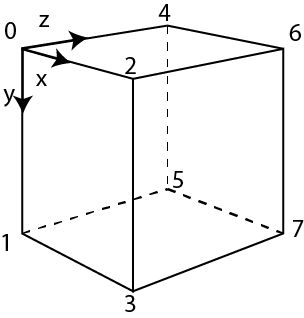
\includegraphics{Illustrations/i3elviscube.png}
    \caption{Illustration of the faces of the cube referred to in Tables \ref{tbl:box_parameters} and \ref{tbl:t_box_parameters}.}
    \label{fig:cube}
\end{figure}

\begin{table}[H]
\centering
\begin{tabular}{l l l}
\toprule
Parameter		& Description			& Range of value \\
\midrule
Type			& Rock type				& $0-140$\\
$[x_0,y_0,z_0]$ & front upper left\\ 
$[x_1,y_1,z_1]$ & front lower left \\  
$[x_2,y_2,z_2]$ & front upper right \\ 
$[x_3,y_3,z_3]$ & front lower right \\ 
$[x_4,y_4,z_4]$ & back upper left \\  
$[x_5,y_5,z_5]$ & back lower left \\ 
$[x_6,y_6,z_6]$ & back upper right \\  
$[x_7,y_7,z_7]$ & back lower right \\ 
\bottomrule
\end{tabular}
\caption{Box parameters}
\label{tbl:box_parameters}
\end{table}

Coordinates can be given either relative [0,1], or absolute [m0, mMAXSIZE], where MAXSIZE cannot be larger than the maximum domain size in this direction. With the leading 'm', the value is interpreted as an absolute value in meters.

e.g.
\begin{lstlisting}
/Type=RockType
/Type__x0__y0__z0___x1__y1__z1_____x2__y2__z2_____x3__y3__z3
/_____x4__y4__z4___x5__y5__z5_____x6__y6__z6______x7__y7__z7
/Asthenosphere
10____0_m15000_0___0__1.1__0_____1.1_m15000_0_____1.1_1.1__0
______0_m15000_1___0__1.1__1_____1.1_m15000_1_____1.1_1.1__1
\end{lstlisting}

\subsubsection{Temperature box description}
Arbitrary shapes of cubes are prescribed by setting the (x,y,z) coordinate of each of the 8 corners (Figure \ref{fig:cube}).

\begin{table}[H]
\centering
\begin{tabular}{l l}
\toprule
Parameter		& Description\\
\midrule
Type			& Box type: $0$ - simple box; $1\&4$ - age box; $5\&6$ - transitional\\
$[x_0,y_0,z_0]$ & front upper left\\
$[x_1,y_1,z_1]$ & front lower left with $x_1=x_0$, $z_1=z_0$\\
$[x_2,y_2,z_2]$ & front upper right with $z_2=z_0$\\ 
$[x_3,y_3,z_3]$ & front lower right with $x_3=x_2$, $z_3=z_0$\\ 
$[x_4,y_4,z_4]$ & back upper left with $x_4=x_5$, $z_4=z_7$\\  
$[x_5,y_5,z_5]$ & back lower left with $z_4=z_7$\\ 
$[x_6,y_6,z_6]$ & back upper right with $x_6=x_7$, $z_6=z_7$\\
$[x_7,y_7,z_7]$ & back lower right\\
$t_0$ & simple box: temperature $P_0$; age box: surface temperature\\
$t_1$ & simple box: temperature $P_1$; age box: initial temperature\\
$t_2$ & simple box: temperature $P_2$; age box: thermal diffusivity $\kappa$ in $P_0$\\
$t_3$ & simple box: temperature $P_3$; age box: thermal diffusivity $\kappa$ in $P_2$\\
$t_4$ & simple box: temperature $P_4$; age box: thermal diffusivity $\kappa$ in $P_4$\\
$t_5$ & simple box: temperature $P_5$; age box: thermal diffusivity $\kappa$ in $P_6$\\
$t_6$ & simple box: temperature $P_6$; age box: characteristic diffusion time\\
$t_7$ & simple box: temperature $P_7$; age box: overprinted linear geotherm $[\degree/m]$\\
\bottomrule
\end{tabular}
\caption{Temperature box parameters}
\label{tbl:t_box_parameters}
\end{table}

Coordinates can be given either relative [0,1], or absolute [m0, mMAXSIZE], where MAXSIZE cannot be larger than the maximum domain size in this direction. With the leading 'm', the value is interpreted as an absolute value in meters.

\paragraph{Box type 0: simple box}
The given temperatures are set to the given coordinates and temperature is interpolated linearly within the box.

\paragraph{Box type 1\&4: age box}
Within the given coordinates the temperature is given by conductive cooling in the following way:
\begin{equation}\label{eqs:cond_cooling}
T(y,t)=T_1-(1-erf(\dfrac{y}{2\sqrt{\kappa\tau}}))(T_1-T_0),
\end{equation}
where $\kappa=\dfrac{k}{\rho c_p}$ is the thermal diffusivity interpolated over the corner of the box and $\tau=\dfrac{l^2}{\kappa}$ is the characteristic diffusion time.

\paragraph{Box type 5\&6: transitional box}
No new temperatures are set but existing temperatures at the coordinates of the box corners are read. Those are then interpolated linearly through out the box.

E.g. the continental crust and lithosphere is modelled in a simple box by a geothermal gradient of $\sim17\,K/km$ spanning the whole width of the model and starting at $12\,km$ depth with a surface temperature of $273\,K$, going down to a depth of $90\,km$:
\lstset{basicstyle=\small}
\begin{lstlisting}
/T_BOXES_DESCRIPTION
/Typ__x0________x2_______y0________y1_______y2_______y3_______z0_______
	_x5_______x7_______y4_______y5_______y6_______y7_______z7_______
	t0___t1___t2___t3___t4___t5___t6___t7
/Oceanic_and_continental_geotherms
0    -0.000001 m350001  m12000    m90000   m12000    m90000 -0.000001
	-0.000001 m350001  m12000    m90000  m12000    m90000  1.000001
	273  1595 273  1595 273  1595 273  1595
\end{lstlisting}

\subsection{mode.t3c}

\subsubsection{Timestepping description}

The first/second line gives the filename and type of the initial file.

In the next very large block one timestep corresponds with one line and the data is only valid for one timestep. Seperate timestep parameters are given in table~\ref{tbl:timestep_parameters}.

\begin{table}[H]
\small
\centering
\begin{tabular}{l p{13cm}}
\toprule
Parameter & Description \\
\midrule
SAVEFILE & name of the file (if this name is non-unique, the file will be overwritten without warning) \\
TYPE & file type: b = binary (no other supported) \\
cyc0max & number of iterations \\
maxxystep & maximum change in x,y,z in one timestep  \\
maxtkstep & maximum step size in temperature \ \\
maxtmstep & maximum step size in time \\
nubeg & global lower viscosity cut-off \\
nuend & global upper viscosity cut-off \\
p0koef & Pressure penalty factor 1, Relaxation parameter in Continuity equation \\
p1koef & Pressure update interpolation from coarser multigrid levels \\
p2koef & Pressure penalty factor 2 \todo{???} \\
unused & - \\
multinum &  number of multigrid levels \\
stp1 & number of iterations/ repeats for whole timestep \\
multinum2 & number of multigrid levels 2 \todo{???} \\
\bottomrule
\end{tabular}
\caption{Timestep parameters}
\label{tbl:timestep_parameters}
\end{table}

\subsubsection{General parameters}
The following parameters are mainly used to control the general behaviour of the program.

\begin{table}[H]
\small
\centering
\begin{tabular}{l p{11cm} l}
\toprule
Parameter & Description & Default \\
\midrule
\pcode{loadmod		}&\pcode{ load from data file (1) or set initial conditions (0) }&\pcode{ 1}\\
printmod 	& print information on the monitor, Yes (1)/ No (2) & 1\\
\pcode{crustmod	}&\pcode{ print information on crustthickness in files for each nth timestep; 0 = disable }&\pcode{ - }\\
\pcode{dynamod		}&\pcode{ do dynamo calculations for each nth timestep; 0 = disabled }&\pcode{ - }\\
\pcode{fl0num 		}&\pcode{ number of otput file Names }&\pcode{ - }\\
movemod 	& do velocity-pressure iterations, solve continuity and Stokes equation & 1\\
tempmod 	& do temperature iterations, solve heat transfer equation & 1\\
markmod 	& move markers Y(1-simple,2-Runge-Kutta4)/N(0) & 2\\
gridmod 	& recalculate density and viscosity & 1\\
outgrid 	& marker move out of grid Y(0)/N(1) Orthogonal Only (2) & 2\\
densimod	& mode of  density calculation: 0-constant, 1-PT-dependent, 2-TDbase 3-PT-dependent+WaterTDbase & 3 \\
stp100 		& \todo{???} & 9000 \\
\pcode{CTreset 	}&\pcode{ composition/temperature reset for water/air at $100\,km$ above surface Y(1)/N(0) }&\pcode{ 1 }\\
\pcode{smeltextract}&\pcode{ extract melt when moving markers Y(1)/N(0) } & \pcode{1}\\
\pcode{sthdatabase }&\pcode{ Use of Mars thermodynamic database Y(1) or standard database N(0) } & \pcode{1}\\
p2vmod		& convert each nth prn to vtr /N(0) & 10 \\
filestop 	& number of timesteps to execute before exiting & 50\\
\bottomrule
\end{tabular}
\caption{General parameters}
\label{tbl:mode_general_parameters}
\end{table}

\subsubsection{Erosion and Sedimentation parameters}

\begin{table}[H]
\small
\centering
\begin{tabular}{l p{10cm} l}
\toprule
Parameter & Description & Initial value \\
\midrule
eroslev 	& Erosion level: markers above this depth which are neither sticky air nor water get converted to sticky air & 8000\\
sedilev 	& Sedimentation level: sticky air or water below this depth gets converted to sediments & 20000\\
waterlev 	& Water level: sticky air markers below water level are converted to water and water markers above water level are converted to sticky air & 12000\\
\bottomrule
\end{tabular}
\caption{Erosion and Sedimentation parameters}
\label{tbl:mode_sed_parameters}
\end{table}

\subsubsection{Velocity- and Pressure-iterations parameters}
The following parameters are mainly needed to solve the Continuity and Stokes equation with multigrid. Some these parameters already appeared in table~\ref{tbl:timestep_parameters} and their global value given here will be overwritten with the new value for each timestep. 

\begin{table}[H]
\small
\centering
\begin{tabular}{l p{9cm} p{3cm}}
\toprule
Parameter & Description & Initial value \\
\midrule
cyc1max 	& unused & $3000$\\
DIVVMIN 	& Continuity equation lower error bound & $3e{-03}$\\
STOKSMIN 	& Stokes equation lower error bound & $5e{+01}$\\
DIVVMAX 	& Continuity equation upper error bound & $0e{-03}$\\
STOKSMAX 	& Stokes equation upper error bound & $3e{-03}$\\
multinum 	& number of multigrid levels; overwritten by separate timestep value & $4$\\
multicyc	& Number of whole multigrid V-cycle iterations & $1$ \\
multinnn 	& V-cycle structure: number of GS-iterations for each multigrid level in upcycle and downcycle. & $4\,16\,16\,32\,0$; $4\,16\,16\,32\,64$\\
p0koef 		& Global pressure penalty factor 1, Relaxation parameter in Continuity equation; overwritten by separate timestep value & $3.0e{-01}$\\
p1koef 		& Global pressure update interpolation from coarser multigrid level; overwritten by separate timestep value & $1.0e{-00}$\\
p2koef 		& Global pressure penalty factor 2 \todo{???}; overwritten by separate timestep value & $0.0e{-00}$\\
v0koef 		& Velocity penalty facto. Relaxation parameter in vx-,vy-,vz-Stokes equation & $1.0e{-00}$\\
v1koef 		& \todo{???} & $1.0e{-00}$\\
nubeg 		& global lower viscosity cut-off; overwritten by separate timestep value & $1e{+18}$\\
nuend 		& global upper viscosity cut-off; overwritten by separate timestep value & $1e{+25}$\\
nukoef 		& Average $\nu$ for pressure optimisation & $0.0$\\
viscmod 	& Effective viscosity mode. 0 = lin. interp; 1 = exp. interp; 2 = inverse interp; & $0$\\
\pcode{viscoutermod}&\pcode{viscosity in space/air/water; 1-gradual increase in space, 2-gradual increase in water/air}&\pcode{ $2$}\\
\pcode{spheryn 	}&\pcode{ Spherical gravity. 0 = off; 1 = on; }&\pcode{ $0$}\\
\bottomrule
\end{tabular}
\caption{V and P iterations parameters}
\label{tbl:mode_v_p_parameters}
\end{table}

\paragraph{viscmod: Effective viscosity interpolation}
Type of interpolation done to obtain effective viscosity. viscmod = 0 uses linear interpolation (eq.~\ref{eqs:viscmod0}), viscmod = 1 uses exponential interpolation (eq.~\ref{eqs:viscmod1}) and viscmod = 2 uses inverse interpolation (eq.~\ref{eqs:viscmod2}).
\begin{subequations}
\begin{equation}\label{eqs:viscmod0}
\eta_{eff}=\dfrac{1}{8}\sum_{i}\eta_i
\end{equation}
\begin{equation}\label{eqs:viscmod1}
\eta_{eff}=exp{\left(\dfrac{1}{8}\sum_{i}\left(log\left(\eta_i\right)\right)\right)}
\end{equation}
\begin{equation}\label{eqs:viscmod2}
\eta_{eff}=\dfrac{1}{\frac{1}{8}\sum\limits_{i}{\frac{1}{\eta_i}}}
\end{equation}
\end{subequations}

\subsubsection{Temperature-iterations parameters}
The following parameters are mainly needed to solve the temperature equation with multigrid.

\begin{table}[H]
\small
\centering
\begin{tabular}{l p{9cm} l}
\toprule
Parameter & Description & Initial value \\
\midrule
cyc2max 	& unused & $2500$\\
HEATMIN 	& Temperature equation lower error bound & $1e{-4}$\\
multinumt 	& Number of multigrid levels & $0$\\
multicyct 	& Number of whole multigrid V-cycle iterations & $1$ \\
multittt	& V-cycle structure: number of GS-iterations for each multigrid level in upcycle and downcycle & $1$; $0$ \\
t0koef 		& \todo{???} & $1.0e{-00}$\\
t1koef 		& \todo{???} & $1.0e{-00}$\\
heatdif 	& \todo{???} & $1.0$\\
frictyn 	& \todo{???} & $1$\\
adiabyn 	& \todo{???} & $1$\\
\bottomrule
\end{tabular}
\caption{T iterations parameters}
\label{tbl:mode_t_parameters}
\end{table}

\subsubsection{Hydration and melting parameters}

\begin{table}[H]
\small
\centering
\begin{tabular}{l p{7cm} l}
\toprule
Parameter & Description & Initial value \\
\midrule
tkpor 		& Maximum temperature for porosity & $97300000.0$\\
zmpor 		& Maximum depth for porosity & $75000$\\
vyfluid 	& Initial fluid velocity & $-3e{-09}$\\
vymelt 		& Initial melt velocity & $-3e{-09}$\\
dmwamin 	& Minimum water release difference & $1e{-1}$\\
tdeep 		& \todo{???} & $1880.0$\\
dtdeep 		& \todo{???} & $100.0$\\
drdeep 		& \todo{???} & $000.0$\\
zdeep 		& \todo{???} & $660000.0$\\
vdeep		& \todo{???} & $670000.0$\\
nudeep		& \todo{???} & $1e{+21}$\\
dxwater		& Fluid extension in x & $2e{+3}$\\
dywater		& Fluid extension in y & $2e{+3}$\\
dzwater		& Fluid extension in z & $2e{+3}$\\
maxwater	& Maximum water content in peridotite melt & $5e{-1}$\\
minmelt		& \todo{???} & $1e{-2}$\\
maxmelt		& \todo{???} & $1e{-2}$\\
maxpmelt	& Maximum pressure for dry mantle melting & \\
\bottomrule
\end{tabular}
\caption{Hydration and melting parameters}
\label{tbl:mode_melting_parameters}
\end{table}

\subsubsection{Collision velocity parameters}

Linearly change collision velocity. Use initial constant velocity set from boundary conditions. Between \emph{timebeg} and \emph{timeend} linearly change the collision velocity to the final velocity \emph{velocitykf}.

\begin{table}[H]
\small
\centering
\begin{tabular}{l l l}
\toprule
Parameter & Description & Initial value \\
\midrule
timebeg 	& Begin velocity change & $20e{+6}$\\
timeend 	& End velocity change & $25e{+6}$\\
velocitykf 	& Final collision velocity & $0$\\
\bottomrule
\end{tabular}
\caption{Collision velocity parameters}
\label{tbl:mode_collision_parameters}
\end{table}
% the raw output files .prn
% chapter: prn files

\section{Raw output files: .prn}
Valid for subduction/collision setup

\subsection{Part I: General Information}
\begin{table}[H]
\small
\centering
\begin{tabular}{p{3cm} p{6cm} p{3cm} l}
\toprule
Parameter & Description & Initial value & Unit\\
\midrule
xnumx & Number of nodes in x & $16N+5$ (4 multigrid levels) & - \\
ynumy & Number of nodes in y & $16N+5$ (4 multigrid levels) & - \\
znumz & Number of nodes in z & $16N+5$ (4 multigrid levels) & - \\
mnumx & Number markers per cell in x & - & - \\
mnumy & Number markers per cell in y & - & - \\
mnumz & Number markers per cell in z & - & - \\
xsize & Dimension of model in x & - & $[m]$ \\
ysize & Dimension of model in y & - & $[m]$ \\
zsize & Dimension of model in z & - & $[m]$ \\
pxinit & x-coordinate of initial pressure cell & $(xnumx-1)/2$ & - \\
pyinit & y-coordinate of initial pressure cell & $(ynumy-1)/2$ & - \\
pzinit & z-coordinate of initial pressure cell & - & - \\
pinit & Initial pressure in initial pressure cell & - & $[Pa]$ \\
GXKOEFF & Gravitational acceleration in x & - & $[m/s^2]$ \\
GYKOEFF & Gravitational acceleration in y & - & $[m/s^2]$ \\
GZKOEFF & Gravitational acceleration in z & - & $[m/s^2]$ \\
rocknum & \\
bondnum & \\
marknum & \\
n1 & \\
timesum & Starting time & - & $[years]$ \\
ival1 & \\
gridcur & \\
gridtot & \\
\bottomrule
\end{tabular}
\caption{prn-file general information block}
\label{tbl:prn_general_info}
\end{table}

\subsection{Part II: Rock type information
}
\begin{table}[H]
\small
\centering
\begin{tabular}{l p{8cm} l}
\toprule
Parameter & Description & Unit\\
\midrule
markn0 & Individual lower viscosity limit & $[Pa*s]$ \\ 
markn1 & Individual upper viscosity limit & $[Pa*s]$ \\ 
marks0 & Maximum pore water content & $[\%]$ \\ 
marks1 & Individual upper stress limit (= maximum brittle-ductile transition) & $[Pa]$ \\ 
marknu & Newtonian viscosity & $[Pa^{MM}*s]$ \\ 
markdh & Activation energy & $[J]$\\ 
markdv & Activation volume & $[J/bar]$ \\ 
markss & Dislocation/diffusion creep stress threshold& $[Pa]$ \\ 
markmm & Stress exponent & $(Power)$ \\ 
markll & Pore fluid pressure factor & $(koef)$ \\ 
marka0 & Cohesion & $[Pa]$ \\
marka1 & Cohesion 2 & $[Pa]$ \\
markb0 & Sine of dry friction angle & $[-]$ \\
markb1 & Sine of dry friction angle 2 & $[-]$ \\
marke0 & Lower strain threshold for brittle/ductile transition & $[-]$ \\
marke1 & Upper strain threshold for brittle/ductile transition & $[-]$ \\ 
markro & Density & $[kg/M^3]$ \\ 
markbb & Density koef b & $[1/K]$ \\ 
markaa & Density koef a & $[1/kbar]$\\ 
markcp & Heat capacity  & $[J/kg]$ \\ 
markkt & Thermal conductivity & $[W/(m*K)]$ \\ 
markkf & Temperature dependency koef in conductivity & $[W/(m)]$ \\ 
markkp & Pressure dependency koef in conductivity & $[Pa^{-1}]$ \\ 
markht & heat generation & $[W/kg]$\\ 
\bottomrule
\end{tabular}
\caption{prn-file Rock type information block, see also tbl~\ref{tbl:rock_type_parameters}.}
\label{tbl:prn_rock_type_info}
\end{table}

\subsection{Part III: Nodes information}

For each node the following parameters are given. The order is the following, where $n$ is the number of nodes $nodenum$: $${pr_0,vx_0,...ht_0,pr_1,..,ht_1,..,pr_n,..,ht_n}$$

\begin{table}[H]
\small
\centering
\begin{tabular}{l l p{2cm}}
\toprule
Parameter & Description & Unit\\
\midrule
pr & Pressure & $[Pa]$ \\ 
vx & Velocity in x & $[m/s]$ \\ 
vy & Velocity in y & $[m/s]$ \\ 
vz & Velocity in z & $[m/s]$ \\ 
ro & Density & $[kg/m^3]$ \\ 
nu & Viscosity & $[Pa*s]$ \\ 
tk & Temperature & $[K]$ \\ 
cp & Heat capacity & $[J/kg]$ \\ 
et & Thermal expansivity & $[1/K]$ \\ 
kt & Thermal conductivity & $[Wt/m/K]$ \\
ht  & Heat sources & $[Wt/kg]$ \\
\bottomrule
\end{tabular}
\caption{prn-file Node information block}
\label{tbl:prn_node_info}
\end{table}

\subsection{Part IV: Gridline positions}

\paragraph{Position of gridlines in x direction} $xnumx$ numbers are given
\paragraph{Position of gridlines in y direction }$ynumy$ numbers are given
\paragraph{Position of gridlines in z direction} $znumz$ numbers are given

\subsection{Part V: Boundary Condition Equations}

For each boundary condition there are $5$ values needed. The total number of boundary conditions is $bondnum$. The boundary conditions are all of the following general form:
$$CURPAR = CONST + KOEF1*PAR1$$

\begin{table}[H]
\small
\centering
\begin{tabular}{l p{9cm}}
\toprule
Parameter & Description\\
\midrule
m2 & Index in Indexmatrix bondm\\ 
m3 & Index in BC-matrices, saved in bondm \\ 
bondv1[m3][0] &  $CONST$ value in BC equ. \\ 
bondv1[m3][1] &  $KOEF1$ value in BC equ. \\ 
bondn1[m3] & $PAR1+1$ value in BC equ., $PAR1=0$ means no boundary \\ 
\bottomrule
\end{tabular}
\caption{prn-file boundary condition information block}
\label{tbl:prn_bond_info}
\end{table}

\subsection{Part VI: Markers}

The total number of markers is $marknum$. For each marker the following parameters is given:

\begin{table}[H]
\small
\centering
\begin{tabular}{l p{8cm} l}
\toprule
Parameter & Description & Unit\\
\midrule
markx & Marker position in x & $[m]$\\ 
marky & Marker position in y & $[m]$\\ 
markz & Marker position in z & $[m]$\\ 
markk & Temperature & $[K]$\\ 
markw & Water percentage & $[\%]$\\ 
markd & Density & $[kg/m^3]$\\ 
markex & Accumulated meltfraction & $[\%]$\\ 
marktm & Creation time & $[s]$\\ 
markc1 & Melt composition: Granitic part & $[\%]$\\ 
markc2 & Melt composition: Dacite part & $[\%]$\\
markt  & Rock type & $[nr.]$\\
\bottomrule
\end{tabular}
\caption{prn-file Marker information block}
\label{tbl:prn_marker_info}
\end{table}
% numerical problems and solutions
% chapter: numerical problems and solutions

\section{Numerical problems and solutions}

\begin{enumerate}[-]
%====================================================================================
\item \textit{Program stops because pressure gets too high.}

Solution: This might indicate an awkward or inappropriate model setup. Try to lower the two pressure penalty factors from table~\ref{tbl:timestep_parameters} to $[0.5,0.3,0.1,0.001]$. If that doesn't help, try another model setup.
%====================================================================================
\item \textit{Timestep doesn't converge within the time-limit of the Brutus queue.}

Solution: Use a longer queue, e.g. 24h-queue instead of the 8h-queue. If the problem still persists try one of the following:
\begin{enumerate}[a)]
\item Increase continuity equation error limit DIVMIN in tbl.~\ref{tbl:mode_v_p_parameters} to $3e{-3}$
\item Decrease multinum1 and multinum2 in tbl.~\ref{tbl:timestep_parameters} to $3$.
\item Increase both pressure penalty factors in tbl.~\ref{tbl:timestep_parameters}. Choose something along $[0.05,0.11,0.31,0.41]$.
\item Decrease continuity equation error limit DIVMIN in tbl.~\ref{tbl:mode_v_p_parameters} to $1e{-3}$.
\item Try the following configurations for the pressure penalty factors [p0koef,p1koef,p2koef,p3koef] = $[0.31,1.00,0,0]$ , $[0.41,1.00,0,0]$, $[0.11,0.50,0,0]$
\item Make 4 v-cycles series. In tbl.~\ref{tbl:mode_v_p_parameters} set multicyc = $4$.
\end{enumerate}
%====================================================================================
\item \textit{Unstable model, model goes into very fast convection}

Solution: Try one of the following:
\begin{enumerate}[a)]
\item Decrease maximum timestep \textit{maxtkstep} from $500$ to $100$.
\item Decrease maximum timestep \textit{maxtmstep} from $5e3$ to $1e3$.
\item Increase lower viscosity limit from $10^{18}$ to $10^{19}$.
\end{enumerate}

%===============================================================================
\item \textit{Program stops because of $NaN$ velocities.}


Solution: Try one of the following:

\begin{enumerate}[a)]
    \item In case you are using a low resolution, with few nodes in any direction (< 181), check the amount of cores your job is using on Euler. If this is larger than 2, you are probably getting NaN velocities because of a bug in the solver where parallellisation fails (processors start to compete on coarsest mutligrid levels). Taras says it's in theory fixable, but for now it doesn't work. Try running the job on 2 cores. 
    \item Reconsider the volume balancing. \\
To conserve mass, material coming in needs to be balanced by material going out of the box (air and non-air):
\begin{equation}\label{eqs:fluxes}
    V_{in} = \sum{A_{app} * \Bar{v}}
\end{equation}
where $A_{app}$ is the area where the (average) velocity $\Bar{v}$ is applied. Sticky air surplus or deficits (the net in- or outflow of air) must be compensated by assigning a flux at the upper boundary (deficit divided by area of model box). Likewise, net non-air fluxes must be balanced by in- or outgoing fluxes at the lower boundary, usually with asthenosphere. Especially important in this aspect is if you are using a permeable lower boundary, signified by a $Koef$ of 0.99 in the /Lower\_bondary part of the initfile. In that case, do the following to calculate the flux at the lower boundary:
\begin{enumerate}
    \item Add a virtual 99 nodes to the nodes in the y direction, e.g. 101 -> 200. Your new ysize will be 400 instead of 200 km if you're using a 2 km resolution. 
    \item Calculate the net inflow of non-air material follwing equation \ref{eqs:fluxes}
    \item Divide the net inflow of non-air material by the horizontal surface area (xsize * ysize). This value is the flux at the bottom of the 99 "extra nodes" below the lower boundary
    \item Divide this answer by 100 to get the outflow at the actual lower boundary
\end{enumerate}

\item If you changed the model resolution with respect to your previous setup, check if the external grid uses the new resolution, and don't forget to modify the step100 parameter in \textit{mode.t3c}, which needs to be 4.5 times the x-resolution. 

\end{enumerate}  

\end{enumerate}
% conversion and visualisation with paraview
\input{I3ELVIS_paraview}

% Acknowledgement
%-----------------
%\section*{Acknowledgment}
%\clearpage
%--------------------------------------------------------------


%%%%%%%%%%%%%%%%%%%%%%%%%%%%%%%%%%%%%%%%%%%%%%%%%%%%%%%%%%%%%%%%%%%%%%%%%%%%%%
% References

\addcontentsline{toc}{section}{References}
\bibliography{bib-file}
\clearpage

%%%%%%%%%%%%%%%%%%%%%%%%%%%%%%
% Appendix
%\begin{appendix}
%\input{thesis_appendix}
%\end{appendix}
%%%%%%%%%%%%%%%%%%%%%%%%%%%%%%%%%%%%%%%%%%%%%%%%%%%%%%%%%%%%%%%%%%%%%%%%%%%%%%


\end{document}